
\subsection{3D Kinect Camera Approach}

\subsubsection{Approach Overview}
\label{sec:approachOverview}
An accurate way for gaze tracking is to use the Kinect depth sensing camera so that we track the head pose using 3D data.  The idea is to first build a 3D model of the specific user's head using several frames of the depth images.  Then we can fit the model through rigid transformation onto new frames of depth video stream to estimate the head pose in real-time.  After the head pose is obtained for a depth frame, we transform the corresponding frame of color image to the frontal head pose, and crop out the eye regions for gaze prediction.  This method is more accurate than any 2D non-transforming method for the following reasons.  First, the color image is transformed into a frontal pose, and this transformation introduces minimal distortion to the image given the tracking is good, and makes the eye pose detection much easier and more accurate.  Second, when cropping the eye regions from the color image, we can specify the eye cropping regions ahead of time.  Since all color images are now in frontal pose, the cropping regions remain the same even when the user is rotating his/her head.  This gives a more accurate and more stable cropping.  Of course, the two advantages for this method are both dependent on that the head pose tracking is accurate.

\subsubsection{KinFu Head Modeling}
%what are we trying to achieve
%why do it this way
%open source kinfu, how it works
%what I did to fit it to our purpose
%results achieved
We would like to choose a method for building a user specific 3D model of the head that requires minimal user interactions.  This is because we are focusing on the children with ASD population.  Asking a child with ASD to sit still and keep head straight for a period of time for a 3D laser scanner to scan his/her head is less feasible.  Instead, we aimed to obtain the head model through a short video stream of the Kinect's depth frames captured as the child came into the washroom and stood in front of the sink, without trying to restrict the child's movements.

To achieve this, two pieces of softwares are essential.  One is Point Cloud Library (PCL)'s KinFu, which enables us to integrate the frames from Kinect's depth video stream into a single 3D model of the scene.  The second software is Microsoft Kinect for Windows (K4W) SDK's Skeleton Tracking, which enables us to track where the user's head is, and so that only the head is reconstructed by KinFu.

\paragraph{How KinFu Works}
PCL is an open source stand alone library that processes 3D data in the form of point clouds (collections of 3D points).  It provides functionalities such as filtering, normal estimation, feature extraction, transformations, segmentations, surface reconstructions, etc \cite{rusu20113d}.  KinFu is PCL's open source implementation of Kinect Fusion \cite{pirovano2011kinfu}, an algorithm first proposed by Microsoft and demonstrated in its KinectFusion API in K4W SDK \cite{newcombe2011kinectfusion}.  The idea of Kinect Fusion is related to the traditional Simultaneous Localization And Mapping (SLAM) algorithm \cite{pirovano2011kinfu}, where feature points in the scene are matched across frames of a 2D video stream, so that the camera's orientation within the scene is tracked across frames.  At the same time, the frames are patched together to build a sparse 3D map of the scene.  Kinect Fusion extends SLAM into a dense version where every point in the point cloud now becomes a feature point and the full 3D scene is reconstructed \cite{newcombe2011kinectfusion}. It also makes usage of the General Purposed GPU (GPGPU)'s parallel computation to speed up the algorithm to real-time.  The PCL's KinFu and Microsoft's KinectFusion implementations have similar processing pipeline -- they only differ in some specific low level algorithms used.  Below is KinFu's processing pipeline \cite{newcombe2011kinectfusion}:

\subparagraph{Preprocessing}
First, the depth frame from the Kinect camera is filtered through bilateral filtering to remove noise -- it selectively smooths the surfaces while preserving edges \cite{tomasi1998bilateral}.  The bilateral algorithm's effect is illustrated by Figure \ref{fig:bilateralFiltering}.
\begin{figure} [h]
	\centering
	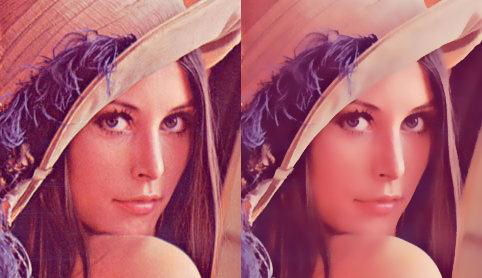
\includegraphics[width=0.6\textwidth]{./img/bilateral_filtering.jpg}
	\caption{A bilateral filter applied to a 2D color image.  The left is the original, while the right is filtered, resulting in removal of noise, figure adapted from \cite{pirovano2011kinfu}}.
	\label{fig:bilateralFiltering}
\end{figure}

If at time \(k\), the raw depth map \( R_k \) gives a depth measurement \( R_k(\textbf{u}) \) at image pixel \( \textbf{u} = (u,v)^T \) in the image domain \( \textbf{u} \in U \), then the bilateral filtered depth map \( D_k \) is given by:
\[  D_k(\textbf{u}) = \frac{1}{W_p} \sum_{\textbf{q} \in U}^{} \mathcal{N}_{\sigma_s}(\| \textbf{u} - \textbf{q} \|_2)  \mathcal{N}_{\sigma_r}(\| R_k(\textbf{u}) - R_k(\textbf{q}) \|_2) R_k(\textbf{q})  \]
, where 
\[ \mathcal{N}_{\sigma}(t) = exp(-t^2 \sigma^{-2}) \]
, and a normalizing constant 
\[  W_p = \sum_{\textbf{q} \in U}^{} \mathcal{N}_{\sigma_s}(\| \textbf{u} - \textbf{q} \|_2)  \mathcal{N}_{\sigma_r}(\| R_k(\textbf{u}) - R_k(\textbf{q}) \|_2)  \] 

After filtering, multiple resolutions of the depth frame is generated through sub-sampling, we call them the multi-resolution pyramid, illustrated by Figure \ref{fig:resolutionPyramid}.  Lastly, each layer of the pyramid generates a 3D point cloud through back projection using the camera's calibration matrix, \(\textbf{K}\), obtaining the point cloud (or vertex map) \(\textbf{V}_k\) in world coordinate,
\[  \textbf{V}_k(\textbf{u}) = D_k(\textbf{u}) \textbf{K}^{-1} \dot{\textbf{u}} \]
, where \( \dot{\textbf{u}} := (\textbf{u}^T|1)^T \)
\begin{figure} [h]
	\centering
	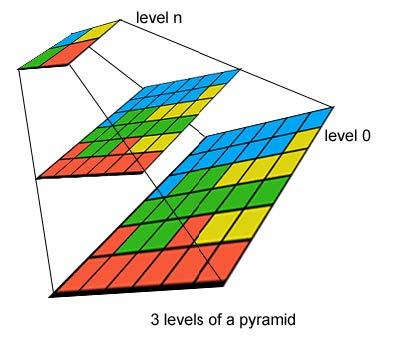
\includegraphics[width=0.6\textwidth]{./img/resolution_pyramid.jpg}
	\caption{A 3-level multi-resolution pyramid, figure adapted from \cite{pirovano2011kinfu}}.
	\label{fig:resolutionPyramid}
\end{figure}

In each point cloud, the normal for each point is estimated by an eigenvector of Principal Component Analysis (PCA) of its neighborhood points \cite{pirovano2011kinfu}.


\subparagraph{Alignment}
The preprocessed point clouds now need to be aligned to the current scene model.  If this is the very first depth frame, then its point cloud is used as the current model -- alignment starts at the second frame.  Alignment is done through the Iterative Closest Point (ICP) algorithm (with some modification of its procedures), starting from the point cloud of the coarsest layer in the pyramid.  ICP is performed in loops until one of the exit criteria is met, after which the same is done for the point cloud of the next level in the pyramid, and the next, until all levels are traversed.

The ICP loop (the modified version) has the following procedures:  Both points from the new frame's point cloud and the model's point cloud are projected to the model point cloud's camera image frame, and any pair of points from the two clouds falling onto the same pixel is noted as a match.  Then the rigid transform that globally minimizes the sum of squared errors between matched points is calculated, the error being the distance between the point of new cloud to the tangent plane of point of the model cloud, seen in Figure \ref{fig:pointToPlaneError} \cite{low2004linear}.
\begin{figure} [h]
	\centering
	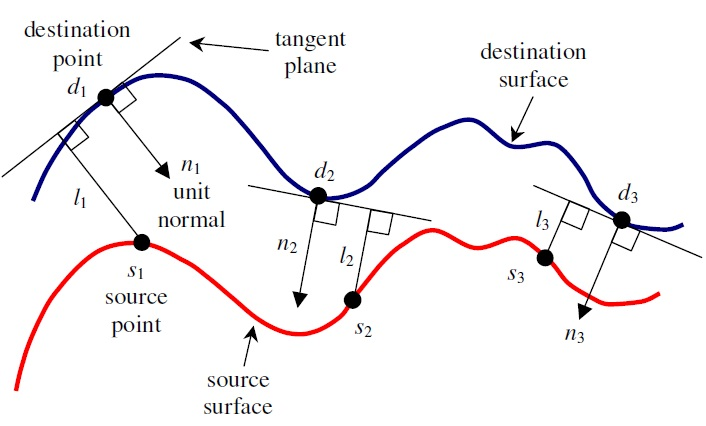
\includegraphics[width=0.6\textwidth]{./img/point_to_plane_error.jpg}
	\caption{Point-to-plane error between two surfaces, figure adapted from \cite{low2004linear}}.
	\label{fig:pointToPlaneError}
\end{figure}


If for a pair of points, \( \textbf{s}_i = (s_{ix}, s_{iy}, s_{iz}, 1)^T \) is the source point, \( \textbf{d}_i = (d_{ix}, d_{iy}, d_{iz}, 1)^T \) is the matched destination point, and \( \textbf{n}_i = (n_{ix}, n_{iy}, n_{iz}, 0)^T \) is the unit normal vector at \( \textbf{d}_i \), then in each ICP loop, the rigid-body transformation matrix \( \textbf{M} \) is found by
\[  \textbf{M}_{opt} = arg min_\textbf{M} \sum_{i}^{} ((\textbf{M} \cdot \textbf{s}_i - \textbf{d}_i) \cdot \textbf{n}_i)^2  \]

The exit criteria for the ICP loop are either 1) the maximum number of iterations are reached, 2) the changes of the transformation matrix falls below threshold, or 3) the sum of squared errors fall below threshold.

\subparagraph{Surface Reconstruction}
Finally, the aligned new frame needs to be integrated into the model and to form a new model point cloud so the pipeline can loop from the top as frames arrive.  A new model point cloud is formed by first converting the two clouds into Truncated Signed Distance Functions (TSDF).  A TSDF is basically a representation of surfaces of objects in a scene, with negative values assigned to voxels inside the surface or voxels that are not measured yet, positive values assigned to voxels outside the surface, increasing in value as we move further away from the surface, and voxels on the surface of objects are assigned the value of zero, illustrated in Figure \ref{fig:TSDF} \cite{newcombe2011kinectfusion}.  Here the raw value of the new frame with no filtering is used for calculating its TSDF to avoid losing details.
\begin{figure} [h]
	\centering
	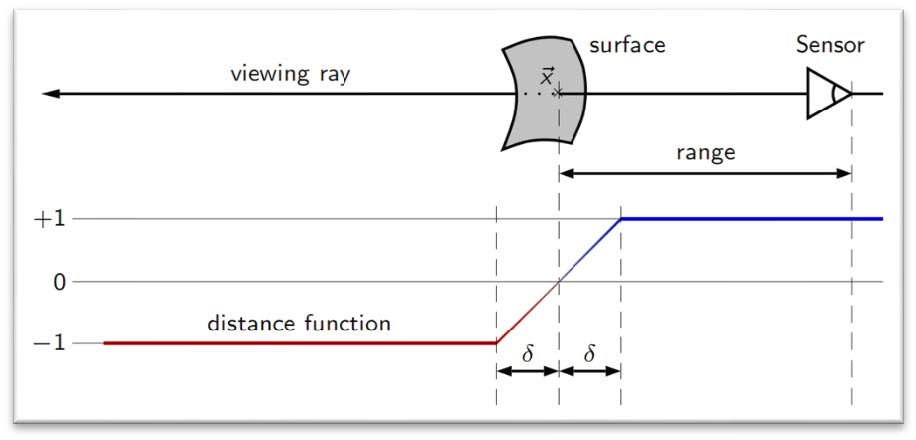
\includegraphics[width=0.6\textwidth]{./img/TSDF.jpg}
	\caption{A illustration of creating an 1D TSDF, figure adapted from \cite{pirovano2011kinfu}}.
	\label{fig:TSDF}
\end{figure}

Specifically, at a point \(\textbf{p}\) in the world coordinate, its projected nearest pixel \(\textbf{x}\) in the depth frame is given by,
\[  \textbf{x} = \lfloor \pi (\textbf{K} \textbf{M}^{-1}_{k} \textbf{p}) \rfloor  \]
, where \( \lfloor.\rfloor \) is the nearest neighbor lookup, and \( \textbf{q} = \pi(\textbf{p}) \) performs perspective projection of \(\textbf{p} = (x,y,z)^T\) with dehomogenization to obtain \(\textbf{q} = (x/z, y/z)^T\).

The TSDF \(F_{R_k}\) of a depth frame \(R_k\) at point \(\textbf{p}\) is computed as,
\[  F_{R_k}(\textbf{p}) = \Psi(\lambda^{-1}\|\textbf{t}_k - \textbf{p}\|_2 - R_k(\textbf{x}))  \]
, \[  \lambda = \|\textbf{K}^{-1} \dot{\textbf{x}} \|_2   \]
, 
\[
\Psi(\zeta) = 
\begin{cases}
min(1, \frac{\zeta}{\mu}) sgn(\zeta)  & \text{iff}\ \zeta \geq -\mu \\
\text{null} & \text{otherwise}
\end{cases}
\]
, where \(\textbf{t}\) is the translation part of the rigid body transformation matrix,
\[  \textbf{M} = 
\begin{bmatrix}
\textbf{R}		&	\textbf{t} \\
\textbf{0}^T	&	1
\end{bmatrix}  \]
, and \(\lambda^{-1}\) converts ray distance from frame origin to \(\textbf{p}\) to a depth value, and \(\Psi(.)\) truncates the SDF to a tolerance \(\mu\) within which distance to the uncertain depth measurement we expect the true value to lie.

After obtaining the TSDFs of the two clouds, volume integration of the two clouds are achieved by a weighted running average of the model cloud's TSDF with the new frame cloud's TSDF.
If the model before integration has TSDF \(F_{k-1}\), then integrating the new frame's TSDF \(F_{R_k}\) gives
\[  F_k(\textbf{p}) = \frac{W_{k-1}(\textbf{p}) F_{k-1}(\textbf{p}) + W_{R_k}(\textbf{p}) F_{R_k}(\textbf{p})} {W_k(\textbf{p})}   \]
\[  W_k(\textbf{p}) = W_{k-1}(\textbf{p}) + W_{R_k}(\textbf{p})  \]
, where \( W_{R_k}(\textbf{p}) \)is the weight used for correcting noisy measurements due to distance from sensor center, and is proportional to \( cos(\theta)/R_k(\textbf{x}) \), \(\theta\) the angle between the direction of the associated pixel ray and the surface normal.

Lastly, surface reconstruction is done through the marching cube algorithm, which converts the new model's TSDF into a point cloud.


%http://research.microsoft.com/pubs/155378/ismar2011.pdf
%http://homes.di.unimi.it/~pirovano/pdf/3d-scanning-pcl.pdf
%http://pointclouds.org/documentation/tutorials/normal_estimation.php

%- KinFu
%	- noise removal via bilateral filtering
%	- creation of multi-resolution pyramid (through sub-sampling)
%	- forming 3D point cloud (through back projection using cameras' calibration matrix) and normal estimation (through eigenvalue estimation) for each layer
%	- alignment (through ICP)
%		- for each point, search, within predefined radius, for its closest point
%		- calculate the rigid transform that minimizes sum of squared distances of all point pairs
%		- repeat this process until
%			- maximum number of iterations reached
%			- difference in transformations fall below threshold
%			- sum of squared distances fall below threshold
%		- KinFu makes modification:
%			- assumes small difference between frames!
%			- in order to parallelize computation, instead of searching for closest point in 3D space, it projects the two clouds onto the first cloud's camera image frame (2D), and pair all points that fall onto the same pixels.
%			- loops through ICP algorithm starting with coarser point clouds first, and works its way down the pyramid
%			- uses point to plane distance metrics instead of point to point, converging faster		
%	- surface reconstruction (through TSDF (Truncated Signed Distance Function) volume integration and marching cube surface reconstruction)
%		- raw depth data is used for merging into model instead of the filtered ones to avoid losing details
%		- calculate TSDF of current model and the new cloud to be merged
%		- merge the two TSDFs using weighted running average
%		- marching cube for reconstructing surface of the updated model's TSDF, creating a smoother point cloud with normals for registering next frame using ICP

\paragraph{Using KinFu with Kinect2 Camera}
To use KinFu with Kinect2 Camera, the open source PCL Kinect2 SDK and PCL Kinect2 KinFu by Steven Hickson (available on GitHub.com) are used.  They act as a driver for Kinect2 camera using the PCL point cloud framework.  This SDK currently only supports generating 3D non-color point cloud from the depth frames of Kinect2.  We had to implement the generation of color point cloud using the color frames ourselves.  However, the advantage of using this over using Microsoft Kinect2 for Windows SDK is that: first, Kinect Fusion was only in an unstable beta version in the Windows SDK during the time this thesis was conducted; second, the open source nature of PCL's KinFu enables us to have much more control in using the algorithm for our application.  The modifications to the KinFu algorithm are outlined in the sections following.


\paragraph{Using KinFu for Head Modeling}
Using KinFu for head modeling is very similar to the original purpose of KinFu -- scene modeling.  The difference lies that, for object (e.g. a head) modeling, we need to filter everything except the object of interest in the depth frame, so that KinFu only builds the 3D model over data on the object, and ignores everything.  One thing that's neat about object modeling is, instead of rotating the Kinect camera around the object, we can rotate the object while fixing the camera.  Also, specifically for head modeling, we can utilize Kinect's Skeleton Tracking algorithm to filter out everything except the head.

Not all objects can be tracked using the ICP algorithm in KinFu.  In KinFu's paper, the author reports that whenever the object is moving too quickly or when not enough 3D features (e.g. edges and corners) are present on the object surface, ICP often fails \cite{pirovano2011kinfu}.  This is mainly due to the assumption in ICP that between frame movements are small (note that this problem may be potentially solved by higher frame rate camera with higher computational power so no frames are skipped).  However, for head tracking, KinFu turns out to work just fine as long as the person isn't moving his/her head too fast.  Shown in Figure \ref{fig:headTrackingResults} (b) is an example 3D mesh model created using the above method.
\begin{figure} [h]
	\centering
	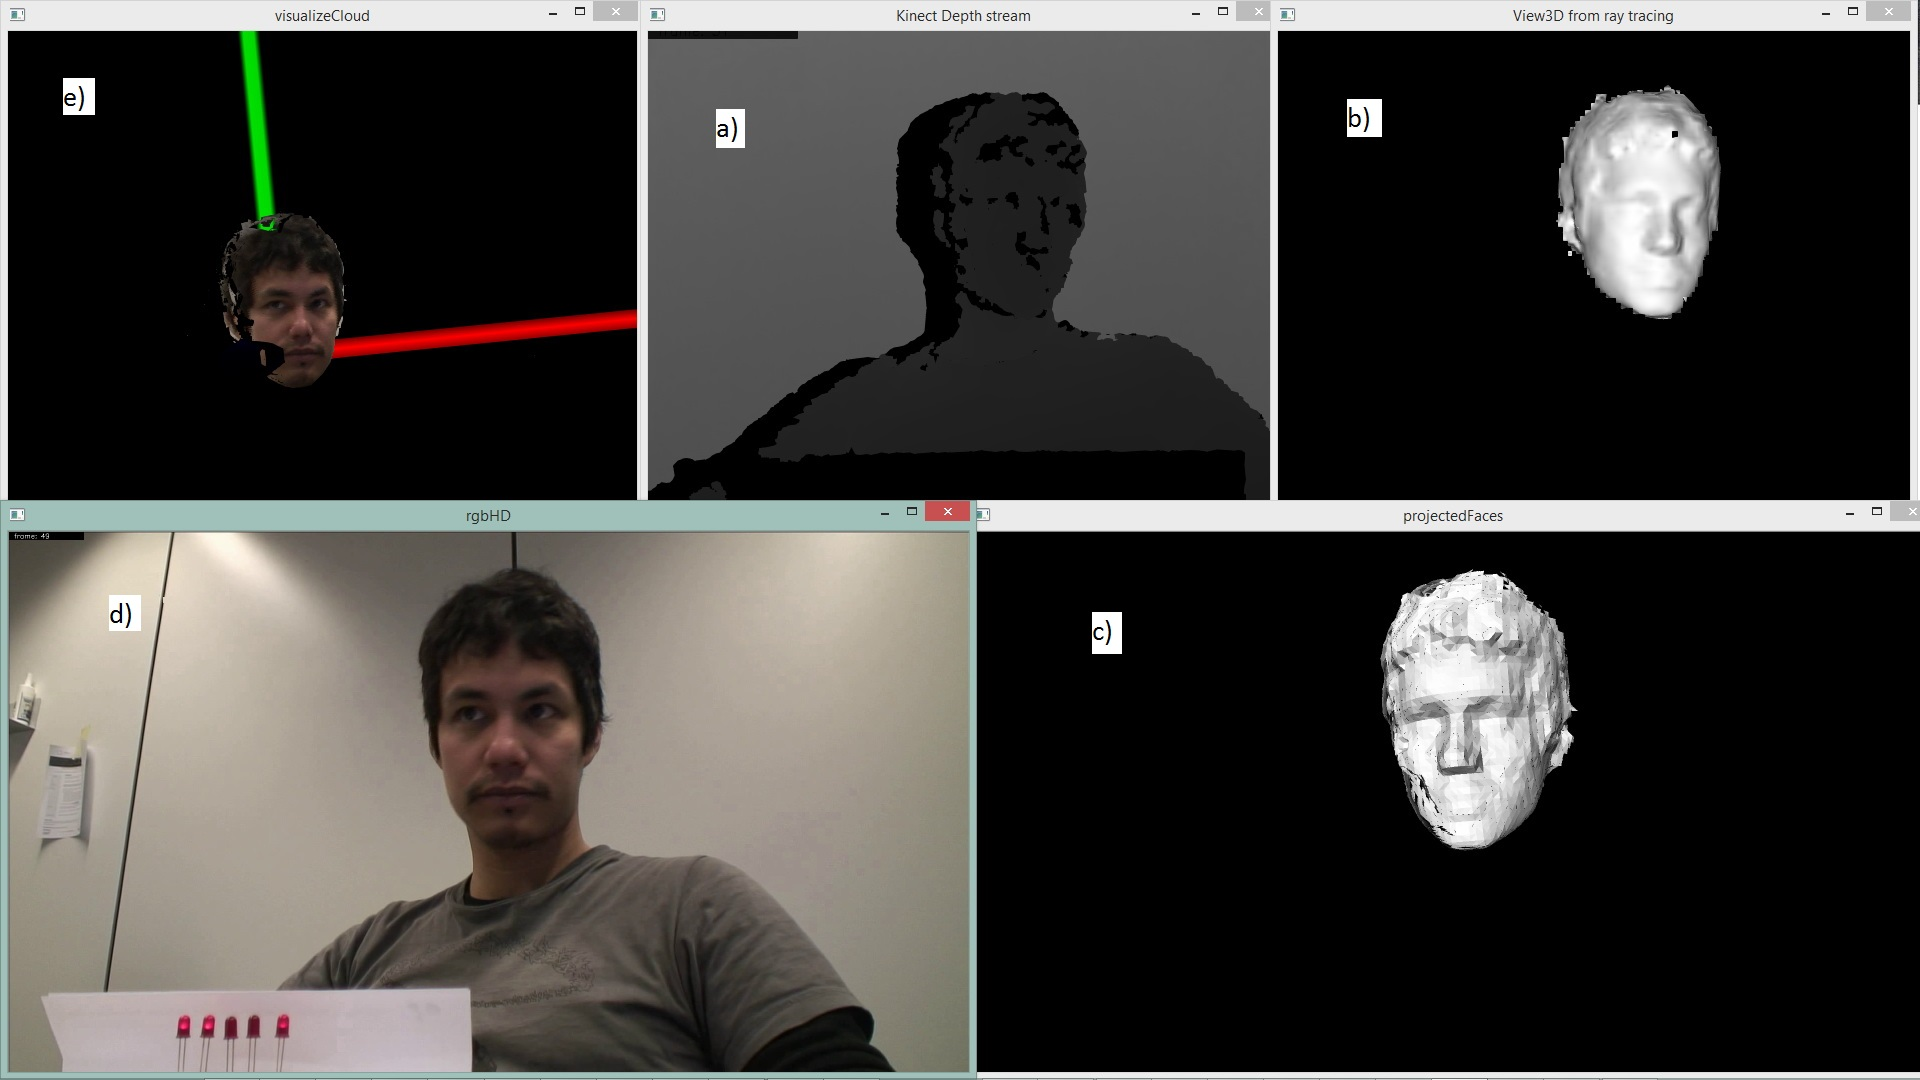
\includegraphics[width=\textwidth]{./img/headTrackingResults1.jpg}
	\caption{The 3D Kinect Camera Approach Results: we start by grabbing a frame from the Kinect depth camera (a), then we fit the 3D head model to the depth frame (b), after which we project the head model mesh onto the color camera image plane (c), so as to associate the color pixels with the head model mesh (d), and lastly forming the 3D color point cloud (e).}
	\label{fig:headTrackingResults}
\end{figure}

Also, facial expressions deform the face, making it deviate from the learned head model, and tracking accuracy may suffer due to the ICP's rigid nature.  Thus we see that the robustness of ICP head tracking depends on two factors:
\begin{itemize}
	\item the head's movement speed (both translational and rotational) relative to the ICP loop process speed or the Kinect camera's frame rate (which ever is the bottleneck)
	\item the dynamics of facial expressions on the head
\end{itemize}

An evaluation of KinFu's capability for head modeling can be done by finding the maximum movement speed of the head (both translational and rotational) under expressionless vs. moving jaw faces conditions before KinFu's alignment step fails.  However, due to limitation of time, the algorithm's capability was not evaluated.


\subsubsection{KinFu Head Pose Tracking}
After obtaining the user's 3D head model, the 3D position and pose (pitch, yaw, and roll) of the head can be tracked in the depth video stream using KinFu.  Skeleton Tracking is again used to filter out everything except the head in the depth video stream.  In addition, it is used to give initial position of head for the ICP loop, so that new frames to be aligned are within the capability of ICP.  Also, the KinFu algorithm needs to be modified to skip the surface reconstruction step, since we already have a model of the head.

A similar evaluation of algorithm capability as mentioned above for KinFu head modeling can be done to see KinFu's robustness in head tracking.  However, this was not conducted due to time limitations.


\subsubsection{Point Cloud Based Inverse Pose Transformation}
Having accurate head model and head pose tracking enable us to restore the color image frames of the user's head into frontal pose.  This inverse pose transformation is done by first forming a colored point cloud from the color frame, then 3D rigid transforming the point cloud inversely to the head pose so that the head represented by the point cloud is in frontal pose, finally projecting the transformed point cloud onto the camera image plane to obtain the 2D color image of the frontal posed head.

\paragraph{Colored Point Cloud}
To form a colored point cloud, we need to calculate the 3D coordinates of every pixel in the color frame.

The function "MapColorFrameToCameraSpace" provided by K4W SDK is for this purpose, and is used by the PCL Kinect2 KinFu SDK by Steven Hickson.  However, MapColorFrameToCameraSpace provides the 3D coordinates of color pixels by associating each pixel in the color frame with a pixel in the depth frame, and then calculating the 3D coordinates of every pixel in the depth frame.  This approach is convenient to code and fast in execution, but is limited by the depth frame resolution.  For the typical resolution of the Kinect2 camera, the color frame resolution is 1920 X 1080 (2073600 pixels), the depth frame resolution is 512 X 424 (217088 pixels).  Using the above method, 2073600 pixels are available in color frame, but can only form 217088 unique points in the point cloud.  This is an order of magnitude reduction, wasting the HD color frame provided by the Kinect2 camera.  For Kinect1 camera, with color frame and depth resolutions being 640 X 480 (307200 pixels), this is also a huge reduction in resolution.  This problem of using the depth frame resolution for point cloud greatly reduces the resolution of the resulting frontal pose color image, making the next step, gaze prediction, less accurate if not much harder.

To avoid resolution reduction, we use the 3D head model instead of the depth frame for calculating the 3D coordinates of each color pixel:

\subparagraph{Head Model Mesh Projection}
To do this, we first generate a triangular mesh version of the 3D head model.  Then we transform the head model mesh to match the pose in the current depth frame (done in previous step).  Next, we project the mesh onto the color camera image plane, keeping track of which pixel each vertex of the mesh lands on.  This enables us to mark which mesh surface each pixel in the projected image belongs to.  More specifically, for each mesh surface in the model, we do a depth first search traverse on the projected image starting with the pixel that one of the surface vertices projects to.  During traverse, we go to the pixel's neighbors one by one (there are eight adjacent neighbors to each pixel) if the pixel itself lies within the projected surface (i.e. inside the triangle formed by the surface's three projected vertices), and stop traversing if the pixel is outside of the projected surface, outside of the image boundary , or is already visited by the traverse.  There are times where two surfaces overlap in their projections -- this happens when one surface obstructs the view of the other (from the camera's point of view).  We handle this by assigning pixels to belong to the mesh surface nearest to the camera's focal point.  The result of this head model mesh projection is shown in Figure \ref{fig:headTrackingResults} (c).

\subparagraph{3D Coordinate Calculation}
After assigning surfaces to every pixel, the pixels' 3D coordinates can be calculated by linearly interpolating from the surface vertices.  To do this, we take advantage of the fact that Barycentric coordinates are preserved during projection of a planar object in 3D onto another plane.  Thus, a point on the 3D mesh surface preserves its Barycentric coordinate after projecting onto the color image plane.  Note that expressing a point in Barycentric coordinates w.r.t. a triangle it is on is basically expressing the point as a linear combination of two of the triangle's edges.  Mathematically, this means the following: Given triangular mesh surface vertices with coordinates P1, P2 and P3 in 3D, projected vertices with coordinates p1, p2 and p3 in 2D, and a point on the mesh surface with coordinate P in 3D, and projected coordinate p in 2D.  The Barycentric coorindate for P w.r.t. {P1, P2, P3} is \( (\lambda1, \lambda2, \lambda3)  \), with \( P = \lambda1 \times P1 + \lambda2 \times P2 + \lambda3 \times P3 \), \( \lambda1 + \lambda2 + \lambda3 = 1 \), and \( \lambda1, \lambda2, \lambda3 > 0 \).  Then, the Barycentric coorindate for the projected point, p, w.r.t. {p1, p2, p3} is also \( (\lambda1, \lambda2, \lambda3)  \), with \( p = \lambda1 \times p1 + \lambda2 \times p2 + \lambda3 \times p3 \).  Using this fact, we can calculate the Barycentric coordinate for each pixel w.r.t. the mesh surface it belongs to, and then calculate the pixel's back projected 3D coordinate using the surface's vertices' 3D coordinates.  An example of a colored point cloud formed using this method is shown in Figure \ref{fig:headTrackingResults} (e).

\paragraph{Inverse Pose Transformation}
With the color point cloud created, we are ready to form a frontal pose color image.  First, we rigid transform the cloud so that the center of the head is at coordinate (0, 0, 2 \( \times\) focal length) and its pose facing the origin.  The reason for 2 \( \times\) focal length is that the image plane is at 1 \( \times\) focal length, and we want the cloud to be a little distance away from the image plane so that the projection looks good inside the image boundaries.  Note that focal length is a programmer defined value used in the next step for perspective projection, and is the distance from image plane to the camera's focal point.

\subsubsection{Projection onto Camera Image Plane}
The last step before obtaining the frontal pose color image is the perspective projection.  For this, we go through every point in the color point cloud and calculate each point's 2D image coordinate.  If two points land in the same pixel, the one closer to the camera's focal point is used.  Several images of inverse pose transformed color point clouds projected onto the camera image plane are shown in Figure \ref{fig:inversePoseResults}.  We see that for moderate range of head poses, the algorithm works great.  However, at extreme range of head poses, distortions of the image and occlusions occur.  The distortion is mainly caused by the inaccuracy in head pose tracking as well as the crudeness of the 3D mesh head model (triangular mesh needs to be quite dense to approximate certain fine curves on the face, e.g. near the eyes).  The occlusion is a natural artifact due to lack of data from the RGB image.
\begin{figure}[h]
	\centering
	\begin{subfigure}[b]{0.32\textwidth}
		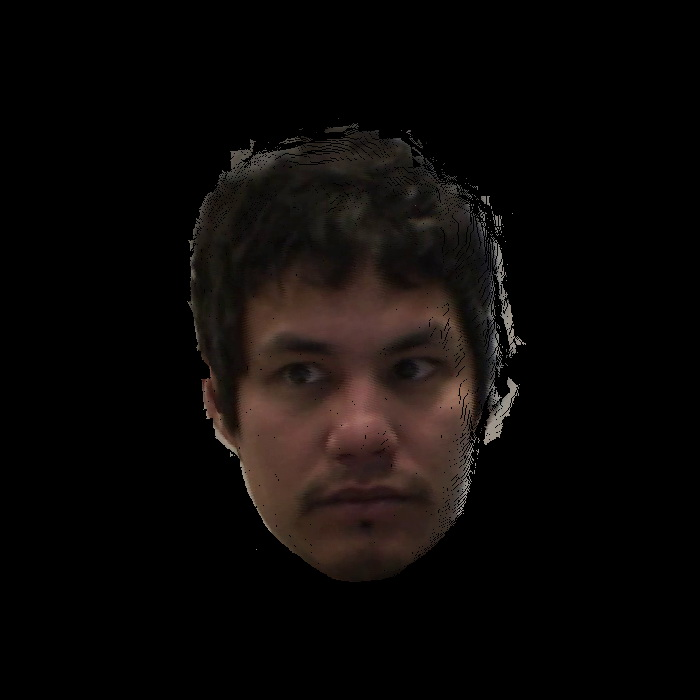
\includegraphics[width=1.1\linewidth]{./img/eyeimages/s1.jpg}
	\end{subfigure}
	\begin{subfigure}[b]{0.32\textwidth}
		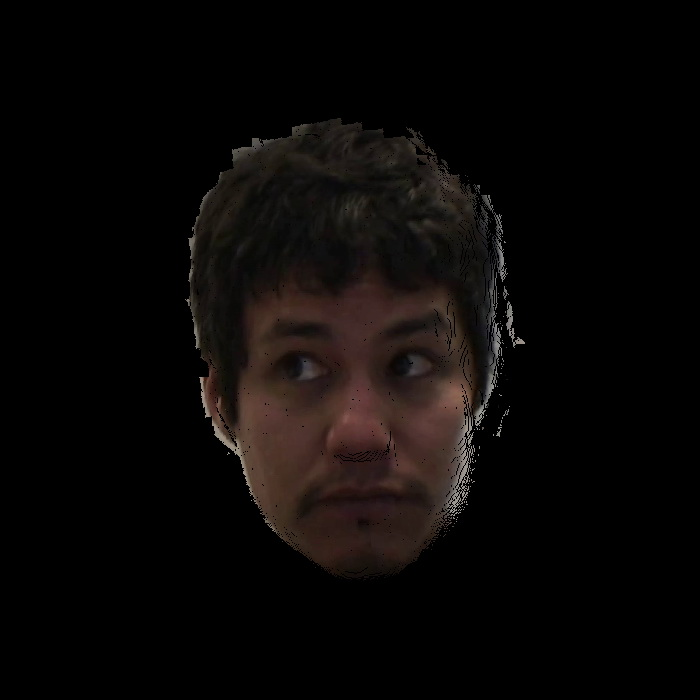
\includegraphics[width=1.1\linewidth]{./img/eyeimages/s2.jpg}
	\end{subfigure}
	\begin{subfigure}[b]{0.32\textwidth}
		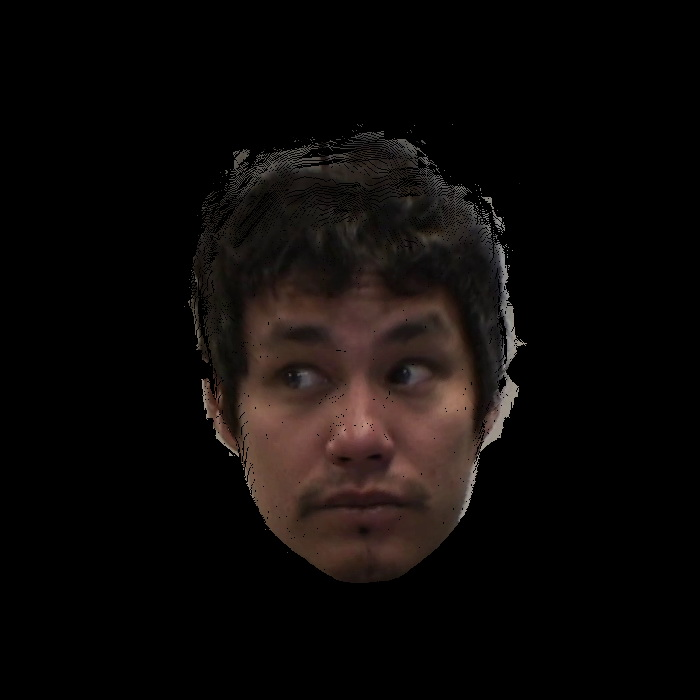
\includegraphics[width=1.1\linewidth]{./img/eyeimages/s3.jpg}
	\end{subfigure}
	\\
	\begin{subfigure}[b]{0.24\textwidth}
		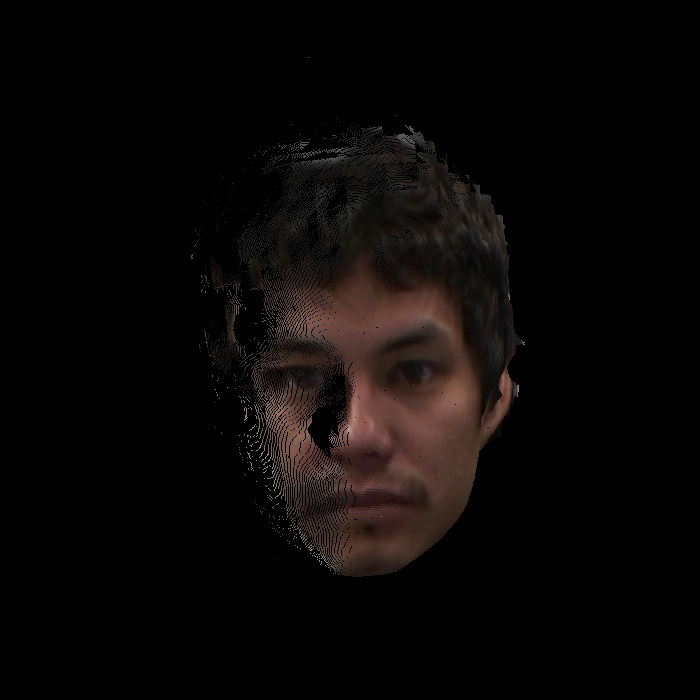
\includegraphics[width=1.1\linewidth]{./img/eyeimages/f1.jpg}
	\end{subfigure}
	\begin{subfigure}[b]{0.24\textwidth}
		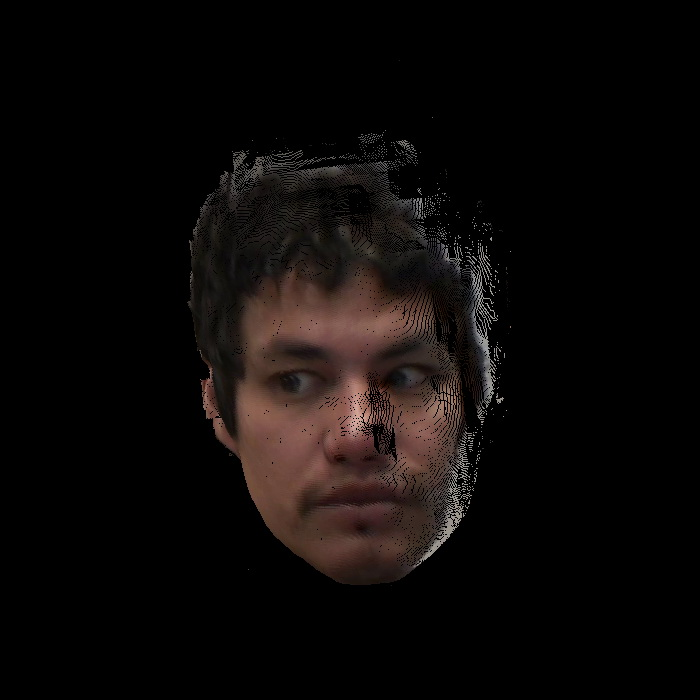
\includegraphics[width=1.1\linewidth]{./img/eyeimages/f2.jpg}
	\end{subfigure}
	\begin{subfigure}[b]{0.24\textwidth}
		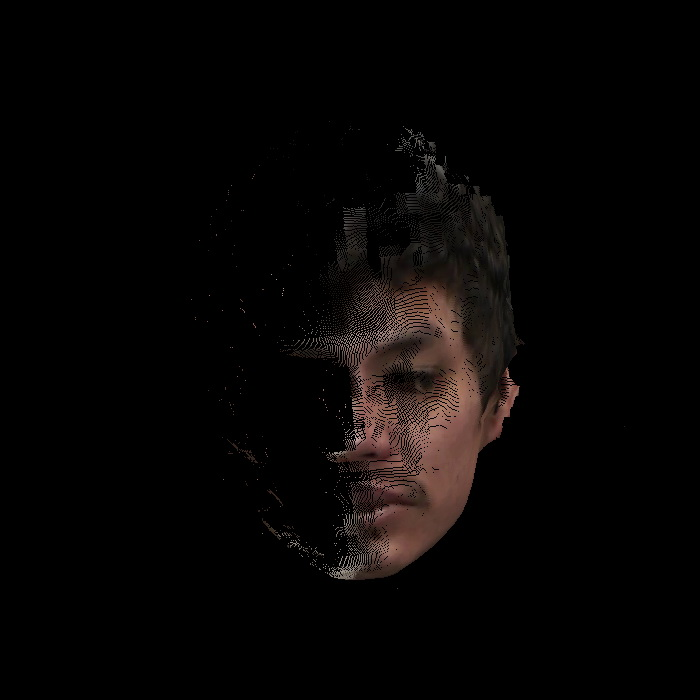
\includegraphics[width=1.1\linewidth]{./img/eyeimages/f3.jpg}
	\end{subfigure}
	\begin{subfigure}[b]{0.24\textwidth}
		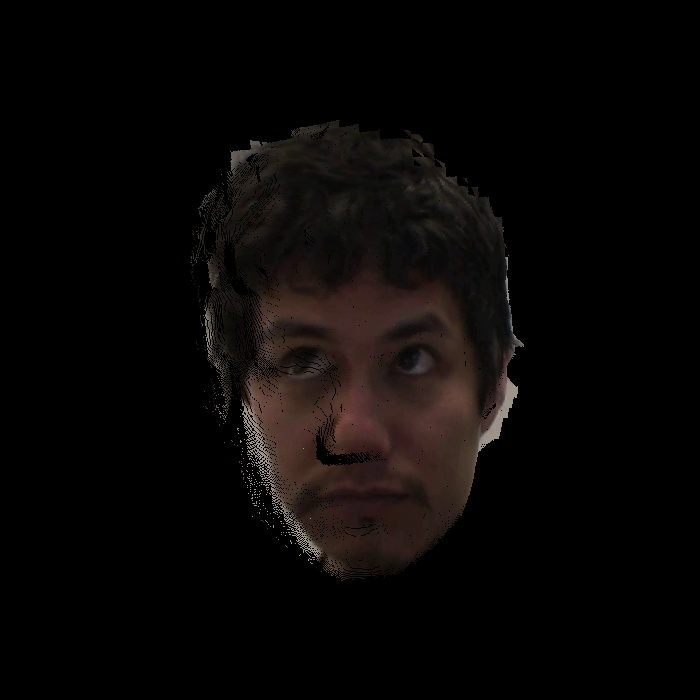
\includegraphics[width=1.1\linewidth]{./img/eyeimages/trackingError.jpg}
	\end{subfigure}
	\caption{Inverse Pose Transformed Color Images of an Example Head: The top row displays images of the head for moderate range of poses, showing little distortion and blank spots; the bottom row displays failure cases, the first three shows extreme head poses resulting in some distortions and huge blank spots due to occlusion, the last image shows a failure case due to head tracking error, resulting in large distortions.}
	\label{fig:inversePoseResults}
\end{figure}


There are pixels in the image that are blank because no points in the color point cloud landed on them.  When the cause of the blank spots is the point cloud being sparse, then the resulting projected image has scattered and small blank spots.  To this end, OpenCV's In-Painting algorithm is used to fill them \cite{bertalmio2000image}.  However, if the blank spots are caused by occlusion due to head pose, the spots are larger and more concentrated, and the In-Painting algorithm may be doing a poor job.  This only happens at the eye regions at extreme head poses, where other sources of distortion errors (e.g. head pose tracking inaccuracy) dominate.  Thus In-Painting being inaccurate in this case is tolerable, and treated as a limitation.

\subsubsection{Using the EYEDIAP Dataset}
Our ultimate goal is to predict the user's gaze given the depth and color video streams from Kinect.  So far, we are able to extract a frontal pose corrected color images of the eye regions.  The next step is to train a gaze predictor so the gaze direction can be predicted given a pair of eye region images.  To this end, we obtained the EYEDIAP Dataset \cite{mora2014eyediap}.

The EYEDIAP Dataset was created by the IDIAP Research Institute for the purpose of training and evaluating gaze prediction algorithms using depth and color video streams.  It consists of 16 participants, 12 males and 4 females.  Participants are asked to gaze follow visual targets while being recorded by a Kinect1 camera and a HD video camera.  For each participant, three visual target conditions are recorded: target on a computer screen changing positions discretely, target on a computer screen changing positions continuously, and a small moving ball floated by a long pole moving continuously.  For each condition, two sessions are recorded, with one requiring the participant's head to remain still while the other allowing free movement.  The videos are annotated automatically for head pose and gaze direction.  This is done by using the 3D Morphable Model (3DMM) algorithm for head tracking, knowing the location of the visual targets on screen, and extracting the location of the floating ball target from the depth data.  Using the annotations, gaze predictors can be trained and evaluated.

To use the EYEDIAP Dataset in our framework, further modifications to the KinFu algorithm were made.  First, instead of subscribing to the video sources of a Kinect camera, the depth and color videos of the dataset are read frame by frame using OpenCV.  Note that we are not using the Kinect1 camera's color videos; instead, the higher resolution HD camera videos are used along with the Kinect1's depth videos.  Depth frames are undistorted using the distortion calibration values provided, following the method used in the open source calibration toolbox by \cite{herrera2012joint}.  Also, image buffers' sizes are changed to match the HD video camera's resolution (1920 X 1080) and the Kinect1 depth camera's resolution (640 X 480).  Next, to form color point clouds, we need to map from depth frame's image coordinate to the world coordinate for forming the face model, and map from the world coordinate to the color frame's image coordinate for assigning mesh surfaces to color pixels.  These mappings are done by transforming the coordinates using the cameras' extrinsics and intrinsics provided.  During processing, the ICP alignment loop along with the color point cloud formation and projection reside in one thread, while the video frames grabbing reside in a separate thread.  Thus, synchronization is needed between threads to ensure no frame skipping when the processing thread is slow.  Lastly, Skeleton Tracking is only available if a dataset is recorded using Kinect Studio, thus it is not available in the EYEDIAP dataset.  Instead, we used in its place the 3DMM head pose tracking annotations by frame provided in the dataset.  We only used the translation part of the head tracking, and only needed it for initialization of ICP -- we still rely on ICP for orientation alignment in the first frame as well as full head pose tracking in new frames after that.

The results shown before (Figure \ref{fig:inversePoseResults}) were created using one of the video data in the EYEDIAP Dataset.

%How well does it perform?
%	- head modeling => not good for floating target and stationary head. => need moving head, DS or CS targets
%	- head tracking => fine for all three conditions?  how about moving vs stationary head?
%	- show results of eye regions cropped?



%\subsubsection{Evaluation On Child With ASD Videos}
